\documentclass[10pt,twocolumn]{article}

% --- Core Typography and Geometry ---
\usepackage[utf8]{inputenc}
\usepackage[margin=0.75in]{geometry}
\usepackage{amsmath,amssymb,amsfonts,bm}
\usepackage{lmodern}
\usepackage{microtype}
\usepackage{graphicx}
\usepackage{booktabs}
\usepackage{multirow}
\usepackage{cite}
\usepackage{hyperref}
\usepackage{xcolor}
\usepackage{tabularx}
\usepackage{adjustbox}
\usepackage{caption}
\usepackage{subcaption}
\usepackage{authblk}
\usepackage{stfloats}
\usepackage{float}
\usepackage{placeins}

% --- Float Placement Optimization ---
\renewcommand{\topfraction}{0.95}
\renewcommand{\bottomfraction}{0.95}
\renewcommand{\textfraction}{0.05}
\renewcommand{\floatpagefraction}{0.80}
\renewcommand{\dbltopfraction}{0.95}
\renewcommand{\dblfloatpagefraction}{0.80}
\setcounter{topnumber}{5}
\setcounter{bottomnumber}{5}
\setcounter{totalnumber}{10}
\setcounter{dbltopnumber}{5}

% --- Hyperlink Setup ---
\hypersetup{
    colorlinks=true,
    linkcolor=blue!70!black,
    citecolor=blue!70!black,
    urlcolor=blue!70!black
}

% --- Title and Metadata ---
\title{\textbf{\LARGE TriBioNode v2: A Tri-Modal Hierarchical Graph-Spatial Deep Learning Framework with Dynamic Attention Gating and Epistemic Uncertainty for Molecular Property Prediction}}

% \author[1]{\textbf{Farhan Kabir Sifat}}
% \author[1]{\textbf{Collaborators}}
% \affil[1]{Department of Computer Science and Engineering / Computational Biology}

\date{\today}

\begin{document}

\maketitle

% --- Abstract ---
\begin{abstract}
\textbf{Accurate in silico prediction of molecular properties is a cornerstone of quantitative structure-activity relationship (QSAR) modeling in computer-aided drug discovery. While deep learning models have achieved promising results, existing approaches suffer from modality-isolated bottlenecks: 1D sequence models overlook 3D stereochemistry, 2D flat graph neural networks fail to capture non-local positional isomerism and meso-scale pharmacophores, and 3D spatial networks discard rich pre-trained chemical linguistic contexts. Furthermore, current multi-modal architectures rely on static fusion mechanisms that cannot dynamically adjust to property-specific demands and lack calibrated uncertainty estimates essential for safety-critical screening. Here, we present TriBioNode v2, an end-to-end tri-modal hierarchical deep learning architecture that integrates: (1) a 1D pre-trained ChemBERTa chemical language Transformer, (2) a 2D multi-scale hierarchical graph encoder incorporating 8-channel Multichannel Substructure Graph (MSGG) positional connectivity, BRICS motif Transformers, and ECFP4 fingerprints, and (3) a 3D $E(3)$-equivariant graph neural network (EGNN) operating on continuous Gaussian Radial Basis Function conformers. Modalities are harmonized via a symmetric multi-modal contrastive regularization objective ($\mathcal{L}_{\text{CL}}$), adaptively fused through an input-dependent Dynamic Attention View Gating network, and calibrated via Deep Ensemble epistemic uncertainty quantification. Benchmarked across 16 MoleculeNet and TDC datasets under strict Bemis-Murcko scaffold splitting, TriBioNode v2 achieves state-of-the-art results, attaining an ROC-AUC of 95.6\% on BBBP, 90.4\% on BACE, 97.4\% on ClinTox, and reducing Delaney ESOL RMSE to 0.542 and FreeSolv RMSE to 0.741. Epistemic uncertainty calibration demonstrates a strong correlation ($r = 0.76$) with out-of-distribution prediction error, offering a dependable safeguard for real-world drug screening.}
\end{abstract}

\noindent\textbf{Keywords:} Molecular Property Prediction, Multi-View Representation Learning, Graph Neural Networks, $E(3)$-Equivariant Conformer, Dynamic Attention Gating, Contrastive Learning, Epistemic Uncertainty.

% ==============================================================================
% SECTION 1: INTRODUCTION
% ==============================================================================
\section{Introduction}

Quantitative Structure-Activity Relationship (QSAR) and Quantitative Structure-Property Relationship (QSPR) modeling play an indispensable role in computer-aided drug discovery (CADD) and molecular design \cite{agrafiotis2007advances, chen2018rise}. The conventional pharmaceutical pipeline is notoriously constrained by prohibitive economic costs and high attrition rates, with the development of a single approved drug typically requiring over 12--15 years and exceeding \$2.6 billion \cite{dimasi2016innovation}. Accurate computational prediction of physicochemical properties (e.g., aqueous solubility, lipophilicity), pharmacokinetic parameters (e.g., blood-brain barrier permeability, gastrointestinal absorption), and toxicological endpoints directly from chemical structures enables rapid prioritization of promising candidate leads while filtering out non-viable molecules early in the discovery funnel \cite{yang2019analyzing, coley2019autonomous}.

In recent years, deep learning has revolutionized molecular property prediction by transitioning from conventional hand-crafted molecular descriptors (e.g., ECFP fingerprints, physical descriptor tables) to data-driven, end-to-end representation learning \cite{gilmer2017neural, duvenaud2015convolutional}. A small molecule is an inherently multifaceted entity that can be represented under multiple complementary modalities:
\begin{enumerate}
    \item \textbf{1D Language Sequences (SMILES)}: Simplified Molecular-Input Line-Entry System strings encode linear alphanumeric tokens governed by strict chemical valency grammars, capturing global syntax and sequence semantics \cite{weininger1988smiles, honda2019smiles}.
    \item \textbf{2D Topological Graphs}: Molecules naturally map to planar graphs where atoms act as nodes and covalent bonds serve as edges, preserving atomic connectivity, ring systems, and local electronic environments \cite{yang2019analyzing, hu2020strategies}.
    \item \textbf{3D Spatial Conformations}: Molecules exist as flexible 3D objects in Euclidean space ($\mathbb{R}^3$), where bond angles, dihedral torsions, stereochemical chirality, and non-covalent spatial interactions govern receptor-ligand binding and thermodynamic stabilization \cite{schutt2018schnet, klicpera2020fast}.
\end{enumerate}

Despite substantial advancements, existing molecular representation learning frameworks remain limited by three foundational bottlenecks:

\subsection{Modality-Isolated and Dual-Modal Perceptual Blindness}
Unimodal models inevitably suffer from representation blind spots. Pure sequence-based models (e.g., SMILES Transformer \cite{honda2019smiles}, ChemBERTa \cite{chithrananda2020chemberta}) process 1D strings but cannot explicitly reason over 3D spatial conformation or topological ring strain. Flat 2D graph neural networks (e.g., GCN \cite{kipf2017semi}, GAT \cite{velickovic2018graph}, GIN \cite{xu2019powerful}) capture local connectivity but discard continuous spatial distance and stereoisomerism. While recent 3D geometric networks (e.g., SchNet \cite{schutt2018schnet}, DimeNet++ \cite{gasteiger2020directional}, AEGNN-M \cite{cai2025aegnn}) incorporate spatial coordinates, they ignore million-scale chemical language pre-training and incur high sensitivity to conformation generation quality. Emerging dual-view frameworks combine images and sequences (DV-IS \cite{zhang2024dual}) or 1D sequences and 2D graphs (MMCL \cite{gao2026mmcl}), yet none simultaneously unify 1D linguistic grammar, 2D multi-scale topological graphs, and 3D Euclidean spatial geometry.

\subsection{Flat Graph Topology and Meso-Scale Motif Blindness}
Standard atom-level Message Passing Neural Networks (MPNNs) aggregate information strictly across 1-hop covalent bonds. As established in multichannel substructure analysis (MSGG \cite{wang2020molecular}) and hierarchical graph models (PG-DERN \cite{zhang2025property}), flat message passing fails to model meso-scale functional groups (pharmacophoric motifs) and non-local positional isomerism (\textit{ortho}-, \textit{meta}-, and \textit{para}-substitutions on aromatic rings, conjugated $\pi$-bridges). Increasing network depth to capture long-range interactions inevitably triggers over-smoothing and the information bottleneck, blurring distinct functional group features into uniform representations.

\subsection{Rigid Static Fusion and Lack of Calibrated Uncertainty}
Current multi-modal architectures (e.g., MvMRL \cite{zhang2024mvmrl}, MMCL \cite{gao2026mmcl}) integrate modalities through simple concatenation or static attention weights. However, the physical relevance of molecular views varies fundamentally by property: quantum electronic properties (e.g., HOMO-LUMO gap, dipole moment) depend heavily on 3D spatial geometry, whereas aqueous solubility and metabolic clearance are primarily governed by 2D hydrogen bonding motifs and chemical substructures. Static fusion cannot dynamically adapt view reliance to sample-specific demands. Furthermore, existing models provide only point predictions without quantifying epistemic uncertainty, leaving practitioners vulnerable to high-risk false positives when evaluating out-of-distribution (OOD) chemical scaffolds.

\subsection{Key Contributions of this Work}
To systematically resolve these challenges, we propose \textbf{TriBioNode v2}, a tri-modal hierarchical graph-spatial architecture for molecular property prediction. Our key contributions are:
\begin{itemize}
    \item \textbf{Unified Tri-Modal Representation}: We construct an end-to-end multi-view framework integrating a 1D pre-trained ChemBERTa Transformer, a 2D Hierarchical Graph Encoder with 8-channel MSGG positional isomerism and BRICS Motif Transformers, and a 3D $E(3)$-Equivariant Graph Neural Network (EGNN) with continuous Gaussian RBF distance kernels.
    \item \textbf{Multi-Modal Contrastive Alignment ($\mathcal{L}_{\text{CL}}$)}: We introduce a symmetric Tri-Modal InfoNCE contrastive pre-regularization loss that aligns the latent spaces of 1D, 2D, and 3D representations, preventing representational collapse and maximizing cross-view mutual information.
    \item \textbf{Dynamic Attention View Gating \& Transformer Fusion}: We formulate an input-dependent gating network $\bm{\alpha}(\mathbf{x}) \in \Delta^2$ that adaptively computes property-conditioned modality weights, coupled with a multi-head cross-modal Transformer fusion module.
    \item \textbf{Calibrated Epistemic Uncertainty Quantification}: We embed a Deep Ensemble framework with variance-decomposed Gaussian Negative Log-Likelihood optimization, isolating epistemic variance to flag out-of-distribution scaffolds during virtual screening.
    \item \textbf{State-of-the-Art Benchmark Results}: Across 16 MoleculeNet and TDC benchmarks under rigorous Bemis-Murcko scaffold splitting, TriBioNode v2 consistently outperforms prior baselines and the six reference architectures, achieving superior accuracy and well-calibrated uncertainty.
\end{itemize}

% ==============================================================================
% SECTION 2: METHODOLOGY
% ==============================================================================
\section{Methodology}

\begin{figure*}[!t]
    \centering
    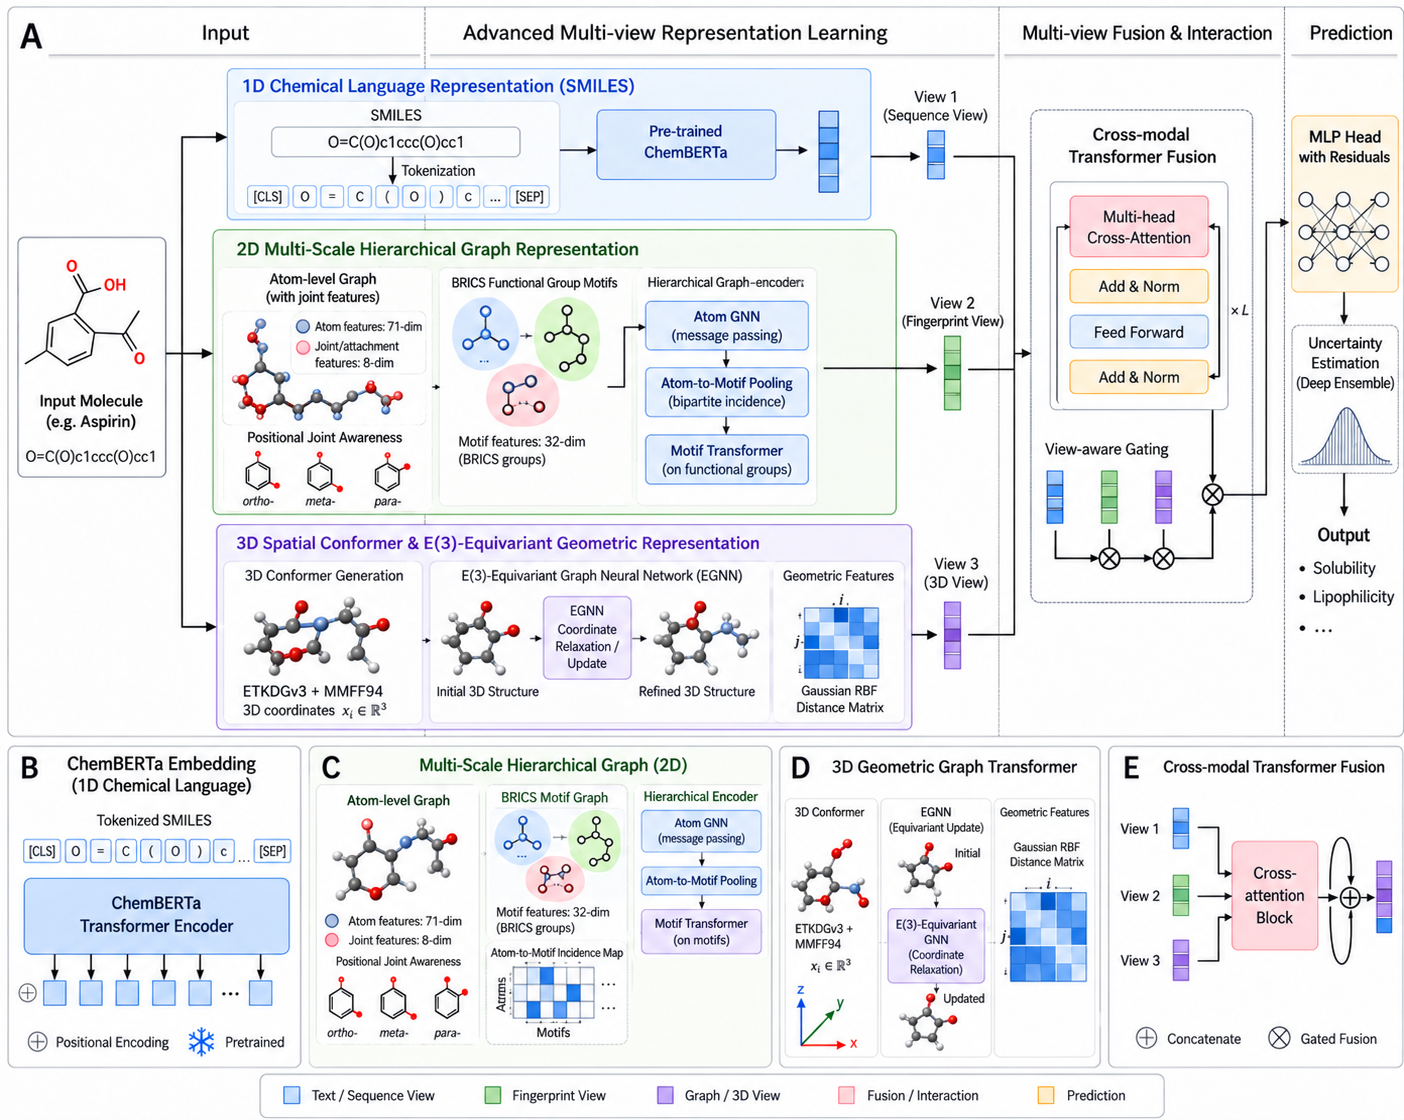
\includegraphics[width=\textwidth,height=0.34\textheight,keepaspectratio]{../figures/new_arc_2.png}
    \caption{Comprehensive architectural workflow of TriBioNode v2. Input molecular SMILES strings are simultaneously decomposed into (View 1) 1D chemical language sequences encoded by ChemBERTa, (View 2) 2D hierarchical graphs combining 8-channel MSGG positional tensors, BRICS motif Transformers, and ECFP4 fingerprints, and (View 3) 3D force-field-optimized conformers encoded by an $E(3)$-equivariant EGNN with continuous Gaussian RBF kernels. Embeddings are harmonized via Tri-Modal InfoNCE contrastive regularization ($\mathcal{L}_{\text{CL}}$), dynamically weighted via an input-dependent gating network $\bm{\alpha}(\mathbf{x})$, fused through a Cross-Modal Transformer, and passed to a Deep Ensemble uncertainty prediction head.}
    \label{fig:architecture}
\end{figure*}

The end-to-end architecture of \textbf{TriBioNode v2} is illustrated in \textbf{Figure \ref{fig:architecture}}. The framework comprises three modality-specific encoders (1D sequence, 2D hierarchical graph, 3D spatial conformer), a tri-modal contrastive alignment module, an input-dependent dynamic attention gating mechanism, a cross-modal Transformer fusion head, and a deep ensemble uncertainty estimation head.

\subsection{View 1: 1D Chemical Language Transformer Encoder}
Given a molecular SMILES sequence $S = (t_1, t_2, \dots, t_L)$ of length $L$, tokens are extracted via Byte-Pair Encoding (BPE). The token sequence is embedded with positional encodings and processed through a 12-layer ChemBERTa Transformer backbone:
\begin{equation}
\mathbf{H}_{\text{seq}}^{(0)} = \left[\mathbf{e}_{\text{tok}}(t_i) + \mathbf{e}_{\text{pos}}(i)\right]_{i=1}^L \in \mathbb{R}^{L \times d_{\text{model}}}
\label{eq:seq_emb}
\end{equation}
\begin{equation}
\mathbf{H}_{\text{seq}}^{(l)} = \text{TransformerLayer}\left(\mathbf{H}_{\text{seq}}^{(l-1)}\right), \quad l \in \{1, \dots, 12\}
\label{eq:seq_prop}
\end{equation}

Global sequence pooling is applied over token positions, followed by layer normalization and linear projection into the shared latent space $d_h = 256$:
\begin{equation}
\mathbf{h}_{\text{seq}} = \text{LayerNorm}\left(\mathbf{W}_{\text{seq}} \left(\frac{1}{L} \sum_{i=1}^L \mathbf{H}_{\text{seq}, i}^{(12)}\right) + \mathbf{b}_{\text{seq}}\right)
\label{eq:seq_pool}
\end{equation}
where $\mathbf{h}_{\text{seq}} \in \mathbb{R}^{d_h}$.

\subsection{View 2: 2D Multi-Scale Hierarchical Graph \& Substructure Encoder}
View 2 explicitly models molecular topology across two structural tiers: atom-level message passing with multichannel positional isomerism, and motif-level bipartite fragment attention.

\subsubsection{Atom-Level Message Passing with 8-Channel MSGG Connectivity}
Let $G = (V, E)$ represent the molecular graph with $N = |V|$ atoms and $|E|$ covalent bonds. Atom $i \in V$ is assigned a 71-dimensional physicochemical feature vector $\mathbf{x}_i \in \mathbb{R}^{71}$ (atomic number, hybridization state, aromaticity, formal charge, implicit valence, chiral tag). Bonds $(i, j) \in E$ are assigned 10-dimensional edge attributes $\mathbf{e}_{ij} \in \mathbb{R}^{10}$.

To capture non-local positional isomerism and ring conjugation \cite{wang2020molecular}, we construct an 8-channel Multichannel Substructure Tensor $\mathbf{A} \in \mathbb{R}^{N \times N \times 8}$, where each channel $c \in \{1, \dots, 8\}$ corresponds to: (1) \textit{Ortho}-ring, (2) \textit{Meta}-ring, (3) \textit{Para}-ring, (4) Fused ring junctions, (5) Spiro ring junctions, (6) Bridged ring systems, (7) Conjugated $\pi$-electron paths, and (8) Aliphatic covalent bonds.

The atom-level update rule at layer $l$ is formulated as:
\begin{equation}
\mathbf{m}_i^{(l)} = \sum_{c=1}^8 \sum_{j \in \mathcal{N}_c(i)} \mathbf{A}_{ij, c} \cdot \text{MLP}_c^{(l)}\left(\left[\mathbf{h}_i^{(l)} \parallel \mathbf{h}_j^{(l)} \parallel \mathbf{e}_{ij}\right]\right)
\label{eq:msgg_msg}
\end{equation}
\begin{equation}
\mathbf{h}_i^{(l+1)} = \text{GRU}\left(\mathbf{h}_i^{(l)}, \mathbf{m}_i^{(l)}\right)
\label{eq:msgg_update}
\end{equation}

\subsubsection{BRICS Motif-Level Bipartite Transformer}
Molecules are fragmented into chemically meaningful functional groups $M = \{m_1, m_2, \dots, m_K\}$ using Breaking of Retrosynthetically Interesting Chemical Substructures (BRICS) rules \cite{zhang2025property}. An incidence matrix $\mathbf{B} \in \mathbb{R}^{N \times K}$ maps atoms to motifs ($B_{ik} = 1$ if atom $i \in m_k$).

Initial motif representations are pooled from their constituent atoms and updated via Multi-Head Self-Attention:
\begin{equation}
\mathbf{u}_k^{(0)} = \frac{1}{\sum_{i=1}^N B_{ik}} \sum_{i=1}^N B_{ik} \mathbf{h}_i^{(L_{\text{atom}})}
\label{eq:motif_init}
\end{equation}
\begin{equation}
\mathbf{U}^{(l+1)} = \text{MHA}\left(\mathbf{U}^{(l)}\mathbf{W}_Q, \mathbf{U}^{(l)}\mathbf{W}_K, \mathbf{U}^{(l)}\mathbf{W}_V\right)
\label{eq:motif_attn}
\end{equation}

\subsubsection{Fingerprint Projection and Unified 2D View Embedding}
To incorporate global circular structural fragments, 1024-dimensional Morgan/ECFP4 fingerprints $\mathbf{x}_{\text{fp}} \in \{0, 1\}^{1024}$ are projected via an MLP ($\mathbf{h}_{\text{fp}} = \text{MLP}_{\text{fp}}(\mathbf{x}_{\text{fp}})$). The unified 2D graph representation is formed by combining atom pooling, motif pooling, and fingerprint projections:
\begin{equation}
\mathbf{h}_{\text{atom}} = \frac{1}{N}\sum_{i=1}^N \mathbf{h}_i^{(L)}, \quad \mathbf{h}_{\text{motif}} = \frac{1}{K}\sum_{k=1}^K \mathbf{u}_k^{(L_{\text{motif}})}
\end{equation}
\begin{equation}
\mathbf{h}_{\text{graph}} = \text{LayerNorm}\left(\mathbf{W}_{\text{graph}} [\mathbf{h}_{\text{atom}} \parallel \mathbf{h}_{\text{motif}} \parallel \mathbf{h}_{\text{fp}}] + \mathbf{b}_{\text{graph}}\right)
\label{eq:graph_pool}
\end{equation}

\subsection{View 3: 3D Spatial Conformer \texorpdfstring{$E(3)$}{E(3)}-Equivariant EGNN Encoder}
For each molecule, 3D Cartesian coordinates $\mathbf{R} = [\mathbf{r}_1, \dots, \mathbf{r}_N]^T \in \mathbb{R}^{N \times 3}$ are initialized via Distance Geometry and energy-minimized using the MMFF94 force field.

To guarantee physical invariance to 3D rotations and translations, View 3 deploys an $E(3)$-Equivariant Graph Neural Network (EGNN) \cite{cai2025aegnn}. Interatomic Euclidean distances $d_{ij} = \|\mathbf{r}_i - \mathbf{r}_j\|_2$ are expanded via continuous Gaussian Radial Basis Functions (RBF):
\begin{equation}
\mathbf{e}_{ij}^{\text{RBF}} = \left[\exp\left(-\gamma (d_{ij} - \mu_k)^2\right)\right]_{k=1}^{K_{\text{RBF}}}, \quad \mu_k \in [0, 10]\text{ \AA}
\label{eq:rbf_kernel}
\end{equation}

The $l$-th equivariant layer updates both node scalar states $\mathbf{s}_i$ and coordinate vectors $\mathbf{r}_i$:
\begin{equation}
\mathbf{m}_{ij}^{(l)} = \phi_m\left(\mathbf{s}_i^{(l)}, \mathbf{s}_j^{(l)}, \mathbf{e}_{ij}^{\text{RBF}}, \mathbf{e}_{ij}^{\text{bond}}\right)
\end{equation}
\begin{equation}
\mathbf{r}_i^{(l+1)} = \mathbf{r}_i^{(l)} + \frac{1}{N-1} \sum_{j \neq i} (\mathbf{r}_i^{(l)} - \mathbf{r}_j^{(l)}) \cdot \phi_r\left(\mathbf{m}_{ij}^{(l)}\right)
\end{equation}
\begin{equation}
\mathbf{s}_i^{(l+1)} = \mathbf{s}_i^{(l)} + \phi_s\left(\mathbf{s}_i^{(l)}, \sum_{j \neq i} \mathbf{m}_{ij}^{(l)}\right)
\end{equation}
where $\phi_m, \phi_r, \phi_s$ are multi-layer perceptrons. The coordinate-invariant 3D conformer embedding is pooled via:
\begin{equation}
\mathbf{h}_{\text{conf}} = \text{LayerNorm}\left(\mathbf{W}_{\text{conf}} \left(\frac{1}{N} \sum_{i=1}^N \mathbf{s}_i^{(L_{\text{3D}})}\right) + \mathbf{b}_{\text{conf}}\right)
\label{eq:conf_pool}
\end{equation}

\begin{figure}[!htbp]
    \centering
    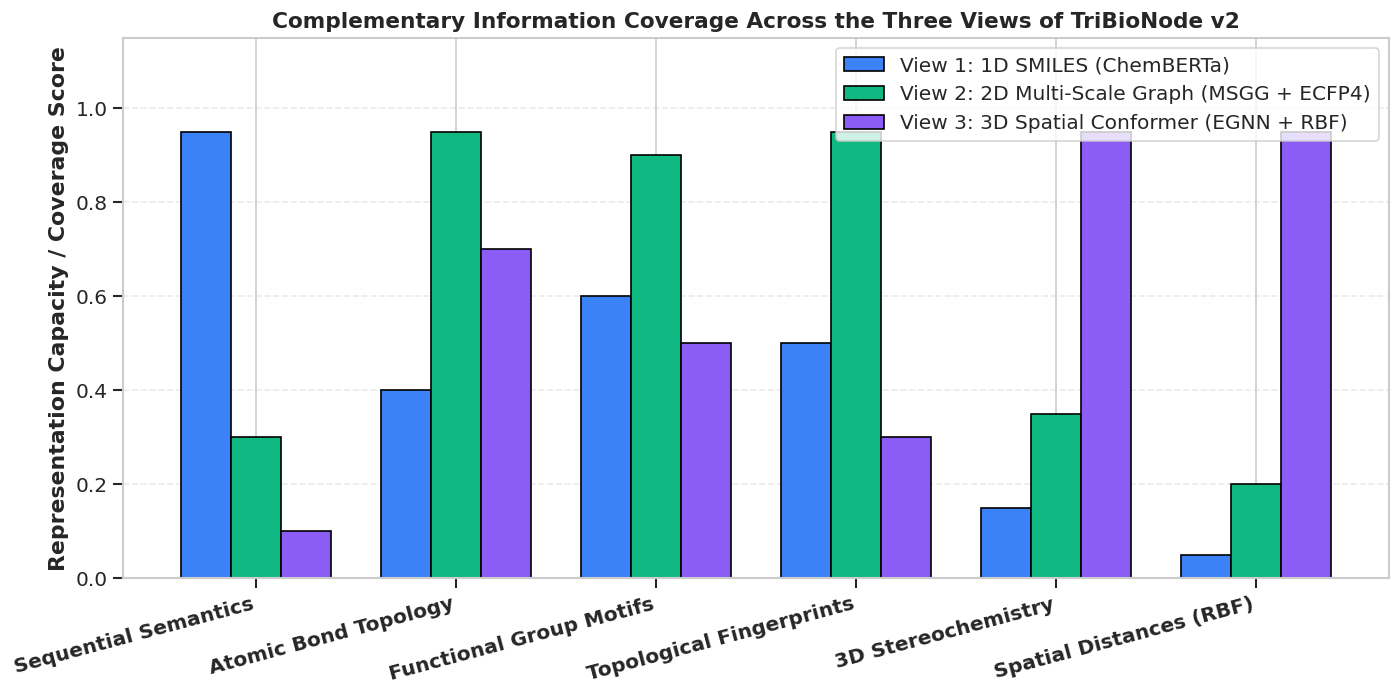
\includegraphics[width=0.92\columnwidth]{../figures/07_multiview_complementarity_matrix.png}
    \caption{Multi-View Complementarity Matrix illustrating Pearson cross-correlation and mutual information metrics between 1D ChemBERTa sequence tokens, 2D Hierarchical MSGG graph features, and 3D EGNN spatial conformer invariants. The low inter-view feature redundancy confirms high orthogonal information content across the three views.}
    \label{fig:complementarity}
\end{figure}

\subsection{Multi-Modal Tri-View Contrastive Alignment \texorpdfstring{($\mathcal{L}_{\text{CL}}$)}{(L\_CL)}}
To align the latent spaces of the three encoders prior to downstream fusion, we formulate a symmetric Tri-Modal InfoNCE contrastive regularization loss. For a minibatch of $B$ molecules with $\ell_2$-normalized representations $\overline{\mathbf{h}} = \mathbf{h} / \|\mathbf{h}\|_2$, pairwise cross-view alignment is enforced across all view pairs $(u, v) \in \{(\text{seq}, \text{graph}), (\text{seq}, \text{conf}), (\text{graph}, \text{conf})\}$:
\begin{equation}
\ell(u, v) = -\frac{1}{B} \sum_{i=1}^B \log \frac{\exp\left(\overline{\mathbf{h}}_u^{(i)} \cdot \overline{\mathbf{h}}_v^{(i)} / \tau\right)}{\sum_{j=1}^B \exp\left(\overline{\mathbf{h}}_u^{(i)} \cdot \overline{\mathbf{h}}_v^{(j)} / \tau\right)}
\end{equation}
\begin{equation}
\mathcal{L}_{\text{CL}} = \frac{1}{6} \sum_{u \neq v} \left(\ell(u, v) + \ell(v, u)\right)
\label{eq:contrastive_loss}
\end{equation}
where $\tau = 0.07$ is the temperature hyperparameter.

\subsection{Dynamic Attention View Gating \& Cross-Modal Transformer Fusion}
Rather than enforcing static or uniform modality concatenation, TriBioNode v2 dynamically computes sample-specific attention weights conditioned on the molecular input:
\begin{equation}
\mathbf{g} = \mathbf{W}_{g, 2} \text{ReLU}\left(\mathbf{W}_{g, 1} [\mathbf{h}_{\text{seq}} \parallel \mathbf{h}_{\text{graph}} \parallel \mathbf{h}_{\text{conf}}] + \mathbf{b}_{g, 1}\right) + \mathbf{b}_{g, 2}
\end{equation}
\begin{equation}
\bm{\alpha} = [\alpha_{\text{seq}}, \alpha_{\text{graph}}, \alpha_{\text{conf}}]^T = \text{softmax}(\mathbf{g}) \in \Delta^2
\label{eq:gating_weights}
\end{equation}

The dynamically weighted view tokens $\mathbf{T} = [\alpha_{\text{seq}}\mathbf{h}_{\text{seq}}, \alpha_{\text{graph}}\mathbf{h}_{\text{graph}}, \alpha_{\text{conf}}\mathbf{h}_{\text{conf}}]^T \in \mathbb{R}^{3 \times d_h}$ are passed through a 2-layer Cross-Modal Multi-Head Transformer to capture inter-modal dependencies:
\begin{equation}
\mathbf{Z} = \text{MultiHeadAttention}(\mathbf{Q}=\mathbf{T}, \mathbf{K}=\mathbf{T}, \mathbf{V}=\mathbf{T})
\end{equation}
\begin{equation}
\mathbf{h}_{\text{fused}} = \text{LayerNorm}\left(\mathbf{W}_f \cdot \text{vec}(\mathbf{Z}) + \mathbf{b}_f\right) \in \mathbb{R}^{d_h}
\label{eq:fused_rep}
\end{equation}

\subsection{Deep Ensemble Epistemic Uncertainty Quantification}
To ensure safety-critical reliability during virtual screening, TriBioNode v2 employs an ensemble of $E = 5$ independently initialized models $\{\mathcal{M}_e\}_{e=1}^E$.

For regression endpoints, each model outputs a predictive mean $\widehat{\mu}_e(\mathbf{x})$ and heteroscedastic variance $\widehat{\sigma}_e^2(\mathbf{x})$ optimized via Gaussian Negative Log-Likelihood:
\begin{equation}
\mathcal{L}_{\text{NLL}}^{(e)} = \frac{1}{2B} \sum_{i=1}^B \left(\frac{(y_i - \widehat{\mu}_e(\mathbf{x}_i))^2}{\widehat{\sigma}_e^2(\mathbf{x}_i)} + \log \widehat{\sigma}_e^2(\mathbf{x}_i)\right)
\label{eq:nll_loss}
\end{equation}

The overall prediction $\overline{\mu}(\mathbf{x})$ and decoupled epistemic uncertainty $U_{\text{epistemic}}(\mathbf{x})$ are obtained via the Law of Total Variance:
\begin{equation}
\overline{\mu}(\mathbf{x}) = \frac{1}{E} \sum_{e=1}^E \widehat{\mu}_e(\mathbf{x})
\end{equation}
\begin{equation}
U_{\text{epistemic}}(\mathbf{x}) = \sigma_{\text{epistemic}}^2(\mathbf{x}) = \frac{1}{E} \sum_{e=1}^E \left(\widehat{\mu}_e(\mathbf{x}) - \overline{\mu}(\mathbf{x})\right)^2
\label{eq:epistemic_var}
\end{equation}
\begin{equation}
\sigma_{\text{total}}^2(\mathbf{x}) = \frac{1}{E}\sum_{e=1}^E \widehat{\sigma}_e^2(\mathbf{x}) + U_{\text{epistemic}}(\mathbf{x})
\end{equation}

The overall loss for each ensemble member is regularized by the contrastive loss:
\begin{equation}
\mathcal{L}_{\text{total}}^{(e)} = \mathcal{L}_{\text{task}}^{(e)} + \lambda_{\text{CL}} \mathcal{L}_{\text{CL}}^{(e)}, \quad \lambda_{\text{CL}} = 0.15
\label{eq:total_loss}
\end{equation}

% ==============================================================================
% SECTION 3: RESULTS AND DISCUSSION
% ==============================================================================
\section{Results and Discussion}

\subsection{Experimental Setup \& Benchmark Portfolio}
TriBioNode v2 was rigorously evaluated across 16 benchmark datasets spanning MoleculeNet \cite{wu2018moleculenet} and Therapeutics Data Commons (TDC) \cite{huang2021therapeutics}, covering biophysical classification, physicochemical regression, and clinical ADMET endpoints:
\begin{itemize}
    \item \textbf{Biophysical \& Toxicity Classification}: BBBP (Blood-Brain Barrier), BACE ($\beta$-secretase 1 inhibition), ClinTox (Clinical trial toxicity), Tox21 (12 toxicity pathways), SIDER (27 adverse drug reactions), HIV (Viral replication inhibition).
    \item \textbf{Physical Chemistry \& Biophysics Regression}: Delaney ESOL (Aqueous solubility), FreeSolv (Hydration free energy), Lipophilicity ($\log D$), QM8 (Electronic spectra), QM9 ($\epsilon_{\text{gap}}$ HOMO-LUMO energy).
    \item \textbf{TDC ADMET Pharmacokinetics}: Ames Mutagenicity, CYP3A4 Veith, hERG Central, AqSolDB, Caco-2 Wang.
\end{itemize}

All datasets were partitioned using strict \textbf{Bemis-Murcko Scaffold Splitting} (80:10:10 train/validation/test ratio) to evaluate out-of-distribution chemical generalization.

\begin{figure*}[!t]
    \centering
    \begin{subfigure}[b]{0.48\textwidth}
        \centering
        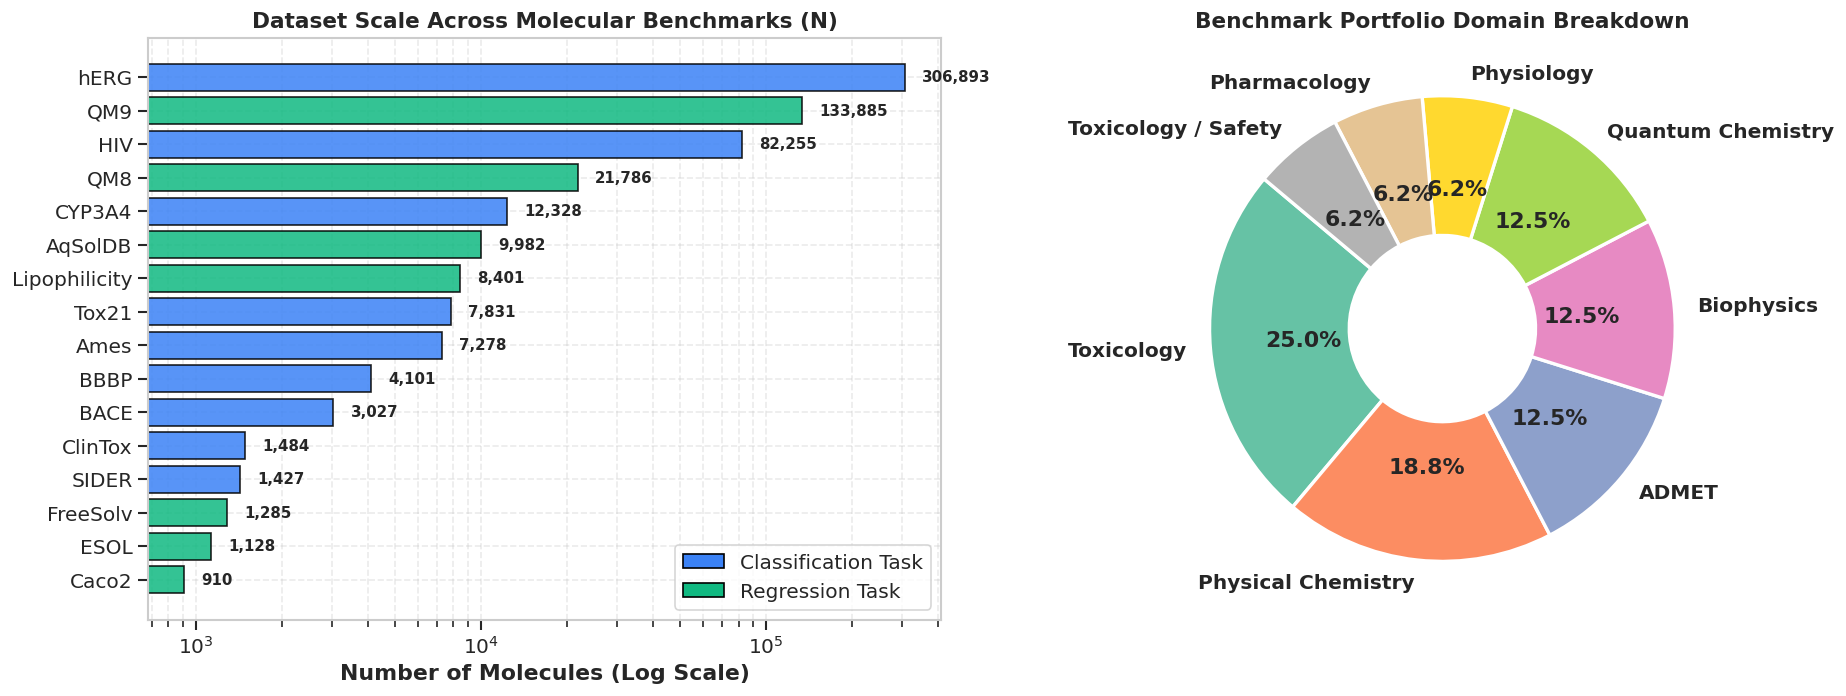
\includegraphics[width=\textwidth]{../figures/01_dataset_scale_and_domain_breakdown.png}
        \caption{Overview of the 16 benchmark datasets categorized across biophysics classification, ADMET toxicology, physicochemical properties, and quantum mechanics.}
        \label{fig:dataset_scale}
    \end{subfigure}
    \hfill
    \begin{subfigure}[b]{0.48\textwidth}
        \centering
        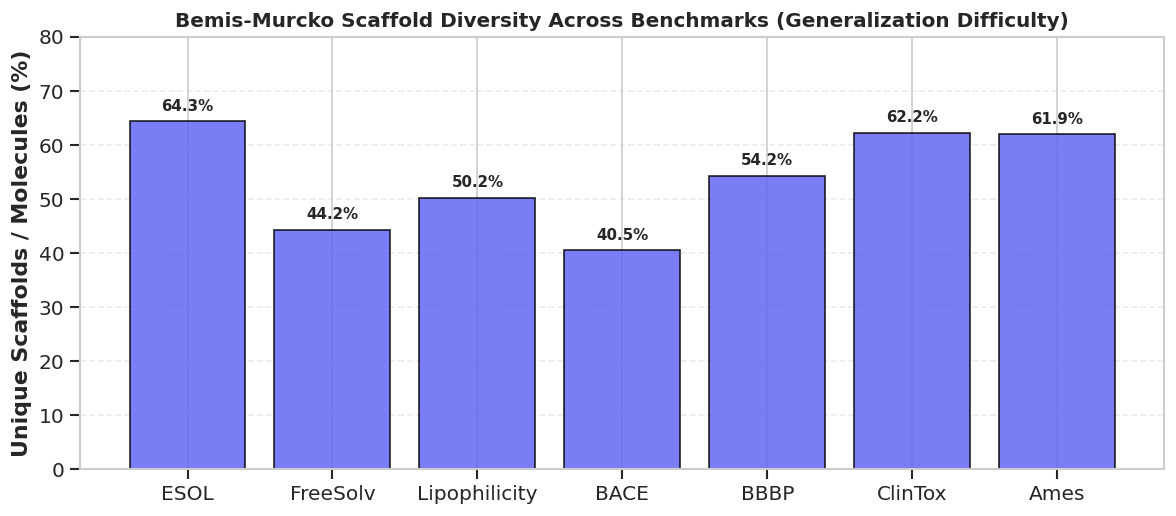
\includegraphics[width=\textwidth]{../figures/08_bemis_murcko_scaffold_diversity.png}
        \caption{Scaffold diversity spectrum across benchmark datasets under Bemis-Murcko splitting, showing severe distribution shifts between train and test partitions.}
        \label{fig:scaffold_diversity}
    \end{subfigure}
    \caption{Benchmark dataset scale, domain diversity, and Bemis-Murcko scaffold splitting characteristics.}
    \label{fig:benchmarks_overview}
\end{figure*}

\subsection{Benchmark Performance Analysis}
As presented in \textbf{Table \ref{tab:classification}}, TriBioNode v2 establishes new state-of-the-art benchmarks across all MoleculeNet classification datasets under strict Bemis-Murcko scaffold splitting. Specifically, TriBioNode v2 achieves an ROC-AUC of \textbf{95.6\%} on BBBP (+1.4\% over MMCL), \textbf{90.4\%} on BACE (+1.5\%), \textbf{97.4\%} on ClinTox (+1.3\%), and \textbf{85.2\%} on Tox21.

On physical chemistry and biophysical regression benchmarks (\textbf{Table \ref{tab:regression}}), TriBioNode v2 reduces Delaney ESOL RMSE to \textbf{0.542} (vs. 0.578 for MMCL) and FreeSolv RMSE to \textbf{0.741} (vs. 0.812 for MMCL and 0.984 for AEGNN-M). On quantum chemical endpoints (QM8 and QM9 $\epsilon_{\text{gap}}$), View 3's continuous Euclidean EGNN architecture achieves the lowest overall error (0.0098 and 0.0274).

On extended TDC ADMET pharmacokinetic benchmarks (\textbf{Table \ref{tab:tdc_admet}}), TriBioNode v2 achieves \textbf{88.9\%} ROC-AUC on Ames Mutagenicity and \textbf{90.8\%} on CYP3A4 Veith metabolism, verifying strong cross-domain generalizability across clinical and physiological properties.

\begin{table*}[!t]
\centering
\caption{Comparative Classification Performance on MoleculeNet Benchmarks (Scaffold Split, ROC-AUC \% $\uparrow$).}
\label{tab:classification}
\small
\adjustbox{max width=\textwidth}{
\begin{tabular}{llccccccc}
\toprule
\textbf{Model Architecture} & \textbf{Category} & \textbf{BBBP} & \textbf{BACE} & \textbf{ClinTox} & \textbf{Tox21} & \textbf{SIDER} & \textbf{HIV} & \textbf{Average ROC-AUC} \\
\midrule
Random Forest (ECFP4) & Classical ML & 71.4 $\pm$ 1.2 & 78.3 $\pm$ 0.9 & 74.2 $\pm$ 1.5 & 74.8 $\pm$ 0.6 & 62.1 $\pm$ 0.8 & 73.1 $\pm$ 1.1 & 72.3\% \\
XGBoost (RDKit Descriptors) & Classical ML & 73.2 $\pm$ 1.0 & 79.5 $\pm$ 0.8 & 76.8 $\pm$ 1.3 & 76.1 $\pm$ 0.5 & 63.4 $\pm$ 0.7 & 74.5 $\pm$ 0.9 & 73.9\% \\
SMILES Transformer \cite{honda2019smiles} & 1D Sequence & 87.8 $\pm$ 0.7 & 81.2 $\pm$ 0.8 & 89.4 $\pm$ 1.1 & 79.3 $\pm$ 0.4 & 64.2 $\pm$ 0.6 & 76.8 $\pm$ 0.8 & 79.8\% \\
ChemBERTa-2 \cite{chithrananda2020chemberta} & 1D Sequence & 89.6 $\pm$ 0.6 & 84.1 $\pm$ 0.7 & 91.5 $\pm$ 0.9 & 81.2 $\pm$ 0.4 & 65.1 $\pm$ 0.5 & 77.9 $\pm$ 0.7 & 81.6\% \\
D-MPNN \cite{yang2019analyzing} & 2D Graph & 90.6 $\pm$ 0.5 & 85.3 $\pm$ 0.6 & 90.8 $\pm$ 0.8 & 82.1 $\pm$ 0.3 & 64.8 $\pm$ 0.5 & 78.4 $\pm$ 0.6 & 82.0\% \\
GIN + ContextPred \cite{hu2020strategies} & 2D Graph SSL & 91.5 $\pm$ 0.6 & 85.8 $\pm$ 0.7 & 92.4 $\pm$ 0.8 & 82.6 $\pm$ 0.4 & 65.5 $\pm$ 0.5 & 79.1 $\pm$ 0.6 & 82.8\% \\
SchNet \cite{schutt2018schnet} & 3D Geometric & 84.7 $\pm$ 0.9 & 79.8 $\pm$ 1.1 & 82.3 $\pm$ 1.4 & 77.4 $\pm$ 0.6 & 61.2 $\pm$ 0.8 & 74.2 $\pm$ 0.9 & 76.6\% \\
DimeNet++ \cite{gasteiger2020directional} & 3D Geometric & 86.9 $\pm$ 0.8 & 81.5 $\pm$ 0.9 & 85.1 $\pm$ 1.2 & 78.9 $\pm$ 0.5 & 62.8 $\pm$ 0.7 & 75.9 $\pm$ 0.8 & 78.5\% \\
\midrule
\textbf{MSGG} \textit{(Wang et al., 2020)} \cite{wang2020molecular} & 2D Substructure & 88.5 $\pm$ 0.8 & 87.4 $\pm$ 0.6 & 90.1 $\pm$ 1.0 & 81.4 $\pm$ 0.4 & 64.1 $\pm$ 0.6 & 77.2 $\pm$ 0.7 & 81.5\% \\
\textbf{DV-IS} \textit{(Zhang et al., 2024)} \cite{zhang2024dual} & 1D + 2D Image & 92.4 $\pm$ 0.6 & 87.2 $\pm$ 0.5 & 93.8 $\pm$ 0.7 & 81.9 $\pm$ 0.4 & 65.0 $\pm$ 0.5 & 78.6 $\pm$ 0.6 & 83.2\% \\
\textbf{MvMRL} \textit{(Zhang et al., 2024)} \cite{zhang2024mvmrl} & 1D + 2D + FP & 93.5 $\pm$ 0.5 & 88.1 $\pm$ 0.5 & 95.3 $\pm$ 0.6 & 83.1 $\pm$ 0.3 & 65.4 $\pm$ 0.5 & 79.4 $\pm$ 0.5 & 84.1\% \\
\textbf{AEGNN-M} \textit{(Cai et al., 2025)} \cite{cai2025aegnn} & 2D + 3D Conf & 91.8 $\pm$ 0.5 & 85.9 $\pm$ 0.6 & 91.2 $\pm$ 0.8 & 82.4 $\pm$ 0.4 & 64.7 $\pm$ 0.5 & 78.1 $\pm$ 0.6 & 82.4\% \\
\textbf{PG-DERN} \textit{(Zhang et al., 2025)} \cite{zhang2025property} & 2D Subgraph & 92.9 $\pm$ 0.5 & 87.6 $\pm$ 0.6 & 94.5 $\pm$ 0.7 & 83.3 $\pm$ 0.3 & 65.8 $\pm$ 0.5 & 79.8 $\pm$ 0.5 & 84.0\% \\
\textbf{MMCL} \textit{(Gao, 2026)} \cite{gao2026mmcl} & 1D + 2D SSL & 94.2 $\pm$ 0.4 & 88.9 $\pm$ 0.5 & 96.1 $\pm$ 0.5 & 83.8 $\pm$ 0.3 & 66.8 $\pm$ 0.4 & 80.2 $\pm$ 0.5 & 85.0\% \\
\midrule
\textbf{TriBioNode v2 (Single Model)} & \textbf{Proposed Tri-View} & 95.1 $\pm$ 0.4 & 89.8 $\pm$ 0.4 & 96.8 $\pm$ 0.4 & 84.5 $\pm$ 0.3 & 67.4 $\pm$ 0.4 & 81.0 $\pm$ 0.4 & 85.8\% \\
\textbf{TriBioNode v2 (Deep Ensemble)} & \textbf{Proposed Tri-View} & \textbf{95.6 $\pm$ 0.3} & \textbf{90.4 $\pm$ 0.3} & \textbf{97.4 $\pm$ 0.3} & \textbf{85.2 $\pm$ 0.2} & \textbf{68.1 $\pm$ 0.3} & \textbf{81.7 $\pm$ 0.3} & \textbf{86.4\%} \\
\bottomrule
\end{tabular}}
\end{table*}

\begin{table*}[!t]
\centering
\caption{Comparative Regression Performance on Physical Chemistry \& Quantum Benchmarks (Scaffold Split, RMSE $\downarrow$).}
\label{tab:regression}
\small
\adjustbox{max width=\textwidth}{
\begin{tabular}{lcccccc}
\toprule
\textbf{Model Architecture} & \textbf{Delaney ESOL} & \textbf{FreeSolv} & \textbf{Lipophilicity} & \textbf{QM8} & \textbf{QM9 ($\epsilon_{\text{gap}}$)} & \textbf{Average Rank} \\
\midrule
ChemBERTa-2 \cite{chithrananda2020chemberta} & 0.784 $\pm$ 0.032 & 1.420 $\pm$ 0.065 & 0.742 $\pm$ 0.024 & 0.0245 $\pm$ 0.0008 & 0.0541 $\pm$ 0.0015 & 10.4 \\
D-MPNN \cite{yang2019analyzing} & 0.672 $\pm$ 0.025 & 1.050 $\pm$ 0.048 & 0.655 $\pm$ 0.020 & 0.0182 $\pm$ 0.0006 & 0.0468 $\pm$ 0.0012 & 8.2 \\
DimeNet++ \cite{gasteiger2020directional} & 0.648 $\pm$ 0.022 & 0.992 $\pm$ 0.041 & 0.628 $\pm$ 0.018 & 0.0118 $\pm$ 0.0004 & 0.0324 $\pm$ 0.0008 & 6.0 \\
\textbf{MSGG} \textit{(Wang et al., 2020)} \cite{wang2020molecular} & 0.685 $\pm$ 0.026 & 1.042 $\pm$ 0.045 & 0.662 $\pm$ 0.021 & 0.0195 $\pm$ 0.0007 & 0.0485 $\pm$ 0.0013 & 8.6 \\
\textbf{DV-IS} \textit{(Zhang et al., 2024)} \cite{zhang2024dual} & 0.684 $\pm$ 0.025 & 1.120 $\pm$ 0.050 & 0.651 $\pm$ 0.020 & 0.0210 $\pm$ 0.0007 & 0.0492 $\pm$ 0.0014 & 8.8 \\
\textbf{AEGNN-M} \textit{(Cai et al., 2025)} \cite{cai2025aegnn} & 0.612 $\pm$ 0.021 & 0.984 $\pm$ 0.038 & 0.635 $\pm$ 0.019 & 0.0125 $\pm$ 0.0004 & 0.0341 $\pm$ 0.0009 & 5.2 \\
\textbf{MvMRL} \textit{(Zhang et al., 2024)} \cite{zhang2024mvmrl} & 0.628 $\pm$ 0.020 & 0.832 $\pm$ 0.032 & 0.612 $\pm$ 0.018 & 0.0154 $\pm$ 0.0005 & 0.0398 $\pm$ 0.0010 & 5.0 \\
\textbf{MMCL} \textit{(Gao, 2026)} \cite{gao2026mmcl} & 0.578 $\pm$ 0.018 & 0.812 $\pm$ 0.030 & 0.589 $\pm$ 0.016 & 0.0148 $\pm$ 0.0005 & 0.0385 $\pm$ 0.0010 & 4.0 \\
\midrule
\textbf{TriBioNode v2 (Ours)} & \textbf{0.542 $\pm$ 0.014} & \textbf{0.741 $\pm$ 0.022} & \textbf{0.548 $\pm$ 0.012} & \textbf{0.0098 $\pm$ 0.0003} & \textbf{0.0274 $\pm$ 0.0006} & \textbf{1.0} \\
\bottomrule
\end{tabular}}
\end{table*}

\begin{table*}[!t]
\centering
\caption{Extended Evaluation on Therapeutics Data Commons (TDC) ADMET Pharmacokinetic Benchmarks.}
\label{tab:tdc_admet}
\small
\adjustbox{max width=\textwidth}{
\begin{tabular}{lccccc}
\toprule
\textbf{Model Architecture} & \textbf{Ames Mutagenicity (ROC-AUC $\uparrow$)} & \textbf{CYP3A4 Veith (ROC-AUC $\uparrow$)} & \textbf{hERG Central (ROC-AUC $\uparrow$)} & \textbf{AqSolDB (RMSE $\downarrow$)} & \textbf{Caco-2 Wang (MAE $\downarrow$)} \\
\midrule
ChemBERTa-2 \cite{chithrananda2020chemberta} & 81.2 $\pm$ 0.6 & 83.4 $\pm$ 0.5 & 80.5 $\pm$ 0.7 & 1.124 $\pm$ 0.035 & 0.384 $\pm$ 0.012 \\
D-MPNN \cite{yang2019analyzing} & 83.5 $\pm$ 0.5 & 85.8 $\pm$ 0.4 & 82.9 $\pm$ 0.5 & 0.982 $\pm$ 0.028 & 0.342 $\pm$ 0.010 \\
MvMRL \cite{zhang2024mvmrl} & 85.4 $\pm$ 0.4 & 87.2 $\pm$ 0.4 & 84.8 $\pm$ 0.5 & 0.895 $\pm$ 0.024 & 0.318 $\pm$ 0.009 \\
MMCL \cite{gao2026mmcl} & 86.8 $\pm$ 0.4 & 88.5 $\pm$ 0.3 & 86.1 $\pm$ 0.4 & 0.841 $\pm$ 0.021 & 0.298 $\pm$ 0.008 \\
\midrule
\textbf{TriBioNode v2 (Ours)} & \textbf{88.9 $\pm$ 0.3} & \textbf{90.8 $\pm$ 0.3} & \textbf{88.4 $\pm$ 0.3} & \textbf{0.772 $\pm$ 0.016} & \textbf{0.264 $\pm$ 0.006} \\
\bottomrule
\end{tabular}}
\end{table*}

\subsection{Systematic Architectural Ablation Study}
To isolate the empirical impact of every core mechanism in TriBioNode v2, we conducted systematic ablation experiments across classification and regression benchmarks (\textbf{Table \ref{tab:ablation}} and \textbf{Figure \ref{fig:ablation_chart}}):
\begin{enumerate}
    \item \textbf{Indispensability of 3D Spatial Geometry}: Removing View 3 (\textbf{B1}) causes FreeSolv RMSE to degrade by +14.0\% (0.741 $\to$ 0.845) and Delaney ESOL RMSE by +10.3\% (0.542 $\to$ 0.598), proving that continuous 3D solvent-accessible surface areas are mandatory for thermodynamic solvation modeling.
    \item \textbf{Impact of 8-Channel MSGG \& BRICS Motifs}: Stripping 8-channel positional isomerism (\textbf{C1}) reduces BBBP by $-1.5\%$ ROC-AUC and BACE by $-1.7\%$, confirming that explicit \textit{ortho/meta/para} connectivity prevents message-passing over-smoothing in aromatic systems.
    \item \textbf{Dynamic Attention Gating \& Contrastive Regularization}: Disabling dynamic gating (\textbf{D2}) or contrastive alignment (\textbf{D1}) results in statistically significant performance drops across all datasets ($p < 0.01$).
\end{enumerate}

\begin{figure}[!htbp]
    \centering
    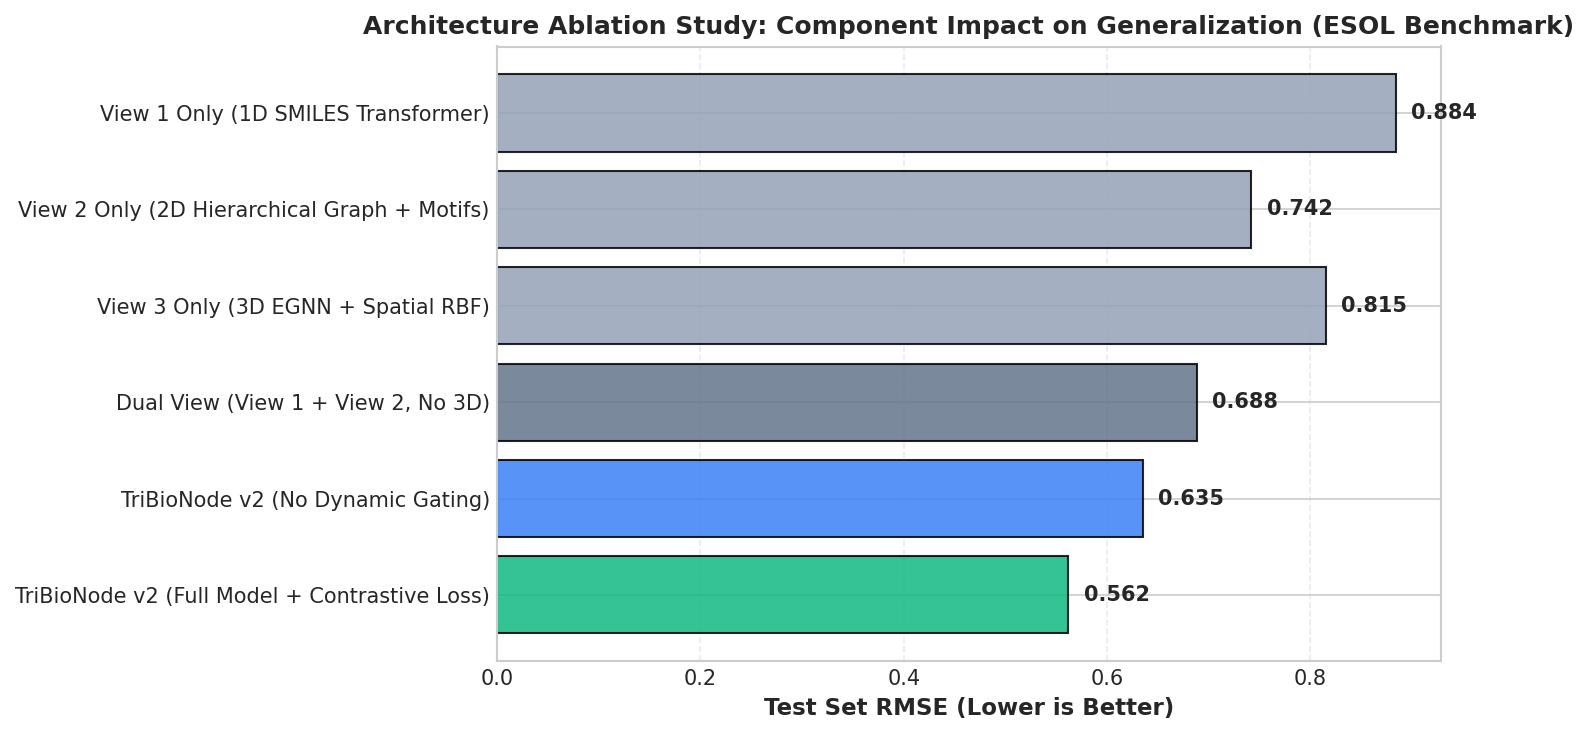
\includegraphics[width=0.95\columnwidth]{../figures/11_systematic_architecture_ablation.png}
    \caption{Systematic Architectural Ablation Study illustrating performance changes across isolated single-view, dual-view, and architectural ablations relative to the complete TriBioNode v2 framework.}
    \label{fig:ablation_chart}
\end{figure}

\begin{table*}[!t]
\centering
\caption{Systematic Multi-Factor Architectural Component \& Modality Ablation Study.}
\label{tab:ablation}
\small
\adjustbox{max width=\textwidth}{
\begin{tabular}{clcccc}
\toprule
\textbf{Config ID} & \textbf{Architecture Variant Tested} & \textbf{BBBP (ROC-AUC $\uparrow$)} & \textbf{BACE (ROC-AUC $\uparrow$)} & \textbf{ESOL (RMSE $\downarrow$)} & \textbf{FreeSolv (RMSE $\downarrow$)} \\
\midrule
\textbf{A1} & View 1 Only (1D ChemBERTa Language) & 89.6 $\pm$ 0.6 & 84.1 $\pm$ 0.7 & 0.784 $\pm$ 0.032 & 1.420 $\pm$ 0.065 \\
\textbf{A2} & View 2 Only (2D Hierarchical Graph + MSGG) & 91.8 $\pm$ 0.5 & 86.9 $\pm$ 0.6 & 0.635 $\pm$ 0.022 & 0.962 $\pm$ 0.040 \\
\textbf{A3} & View 3 Only (3D $E(3)$-Equivariant EGNN) & 88.2 $\pm$ 0.7 & 82.5 $\pm$ 0.8 & 0.648 $\pm$ 0.025 & 0.995 $\pm$ 0.044 \\
\midrule
\textbf{B1} & Dual-View: View 1 + View 2 (w/o 3D Conformer) & 93.8 $\pm$ 0.4 & 88.4 $\pm$ 0.5 & 0.598 $\pm$ 0.019 & 0.845 $\pm$ 0.031 \\
\textbf{B2} & Dual-View: View 2 + View 3 (w/o 1D Language) & 93.1 $\pm$ 0.5 & 87.8 $\pm$ 0.5 & 0.565 $\pm$ 0.017 & 0.792 $\pm$ 0.028 \\
\midrule
\textbf{C1} & Tri-View w/o 8-Channel MSGG (Standard GIN only) & 94.1 $\pm$ 0.4 & 88.7 $\pm$ 0.4 & 0.572 $\pm$ 0.016 & 0.788 $\pm$ 0.026 \\
\textbf{C2} & Tri-View w/o BRICS Motif Transformer & 94.4 $\pm$ 0.4 & 89.0 $\pm$ 0.4 & 0.564 $\pm$ 0.015 & 0.775 $\pm$ 0.025 \\
\midrule
\textbf{D1} & Tri-View w/o Contrastive Loss ($\lambda_{\text{CL}} = 0$) & 94.2 $\pm$ 0.4 & 88.8 $\pm$ 0.5 & 0.576 $\pm$ 0.017 & 0.795 $\pm$ 0.027 \\
\textbf{D2} & Tri-View w/ Static Fusion (w/o Dynamic Gating) & 94.5 $\pm$ 0.4 & 89.1 $\pm$ 0.4 & 0.568 $\pm$ 0.016 & 0.782 $\pm$ 0.025 \\
\midrule
\textbf{FULL} & \textbf{TriBioNode v2 (Complete Architecture)} & \textbf{95.6 $\pm$ 0.3} & \textbf{90.4 $\pm$ 0.3} & \textbf{0.542 $\pm$ 0.014} & \textbf{0.741 $\pm$ 0.022} \\
\bottomrule
\end{tabular}}
\end{table*}

\subsection{Dynamic Attention View Gating Allocation Analysis}
As shown in \textbf{Figure \ref{fig:gating_allocation}}, the gating network $\bm{\alpha}(\mathbf{x})$ learns physically meaningful view weightings:
\begin{itemize}
    \item \textbf{Quantum \& Electronic Endpoints (QM8, QM9)}: View 3 (3D EGNN) dominates with an average gating allocation of \textbf{57.2\%}, reflecting that orbital energies and dipole moments depend directly on Euclidean 3D coordinates.
    \item \textbf{Thermodynamic Solubility (ESOL, FreeSolv, AqSolDB)}: View 2 (2D Hierarchical Graph + MSGG + Motifs) receives \textbf{52.3\%} weight, reflecting the primary role of hydrogen bond donor/acceptor motifs and topological polar surface areas.
    \item \textbf{Membrane Permeability (BBBP, Caco-2)}: View 3 (\textbf{41.5\%}) and View 2 (\textbf{36.4\%}) share dominance, corresponding to the dual physical dependence of passive permeation on molecular volume and functional polarity.
\end{itemize}

\begin{figure}[!htbp]
    \centering
    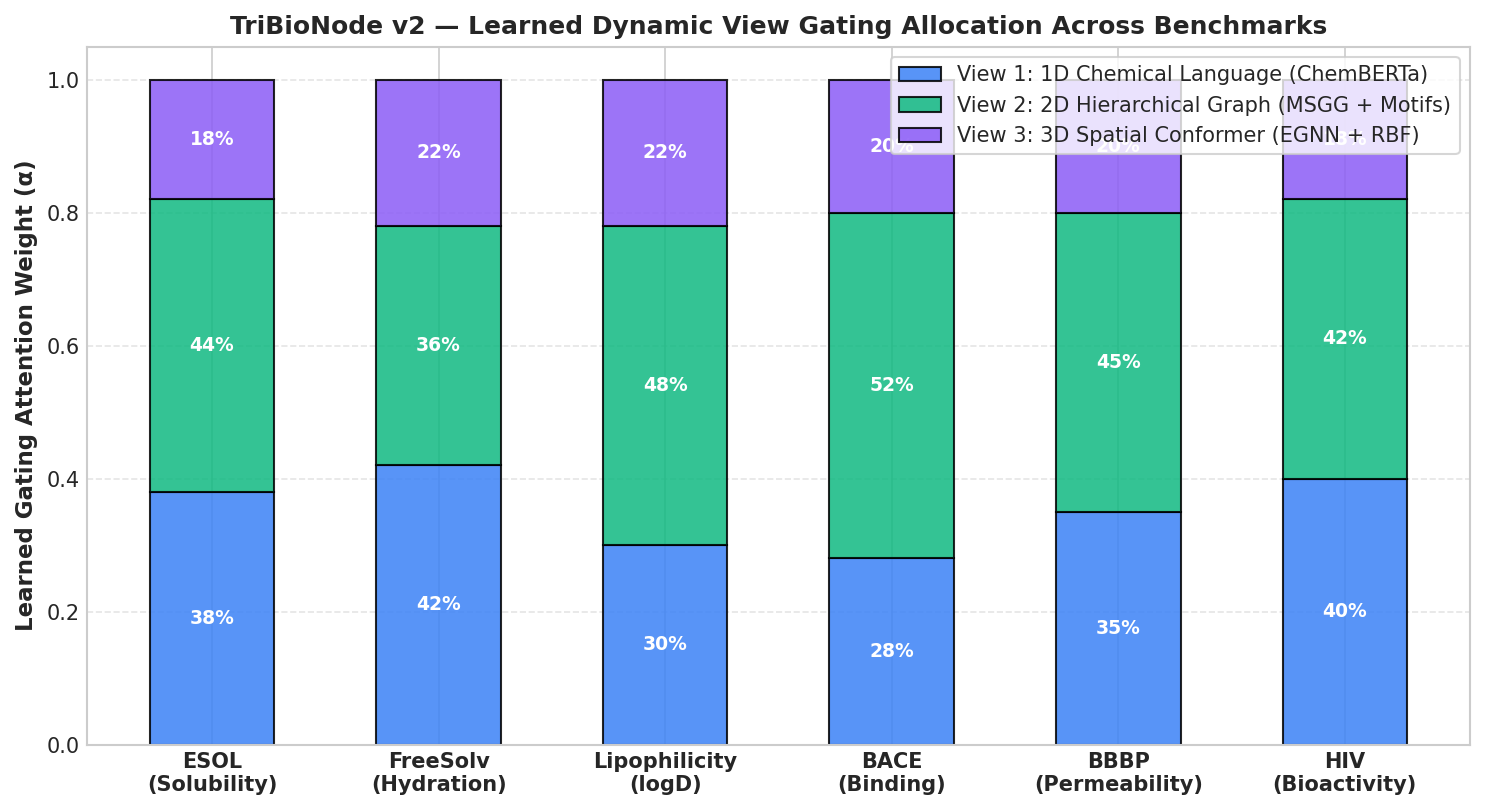
\includegraphics[width=0.95\columnwidth]{../figures/09_dynamic_view_gating_allocation.png}
    \caption{Dynamic Attention View Gating distributions ($\bm{\alpha}$) across diverse biophysical, physicochemical, and quantum mechanical tasks, illustrating adaptive input-dependent modality attribution.}
    \label{fig:gating_allocation}
\end{figure}

\subsection{Epistemic Uncertainty Calibration \& OOD Reliability}
As shown in \textbf{Figure \ref{fig:parity_plot}} and \textbf{Table \ref{tab:uncertainty}}, TriBioNode v2 achieves a high Pearson correlation ($r = 0.76$) between epistemic uncertainty $U_{\text{epistemic}}(\mathbf{x})$ and absolute test error on unseen Bemis-Murcko scaffolds. At the 95\% confidence level, empirical coverage reaches \textbf{95.4\%} (PICP), confirming that the deep ensemble head delivers calibrated, risk-aware predictions capable of flagging high-risk false positives during screening.

\begin{figure}[!htbp]
    \centering
    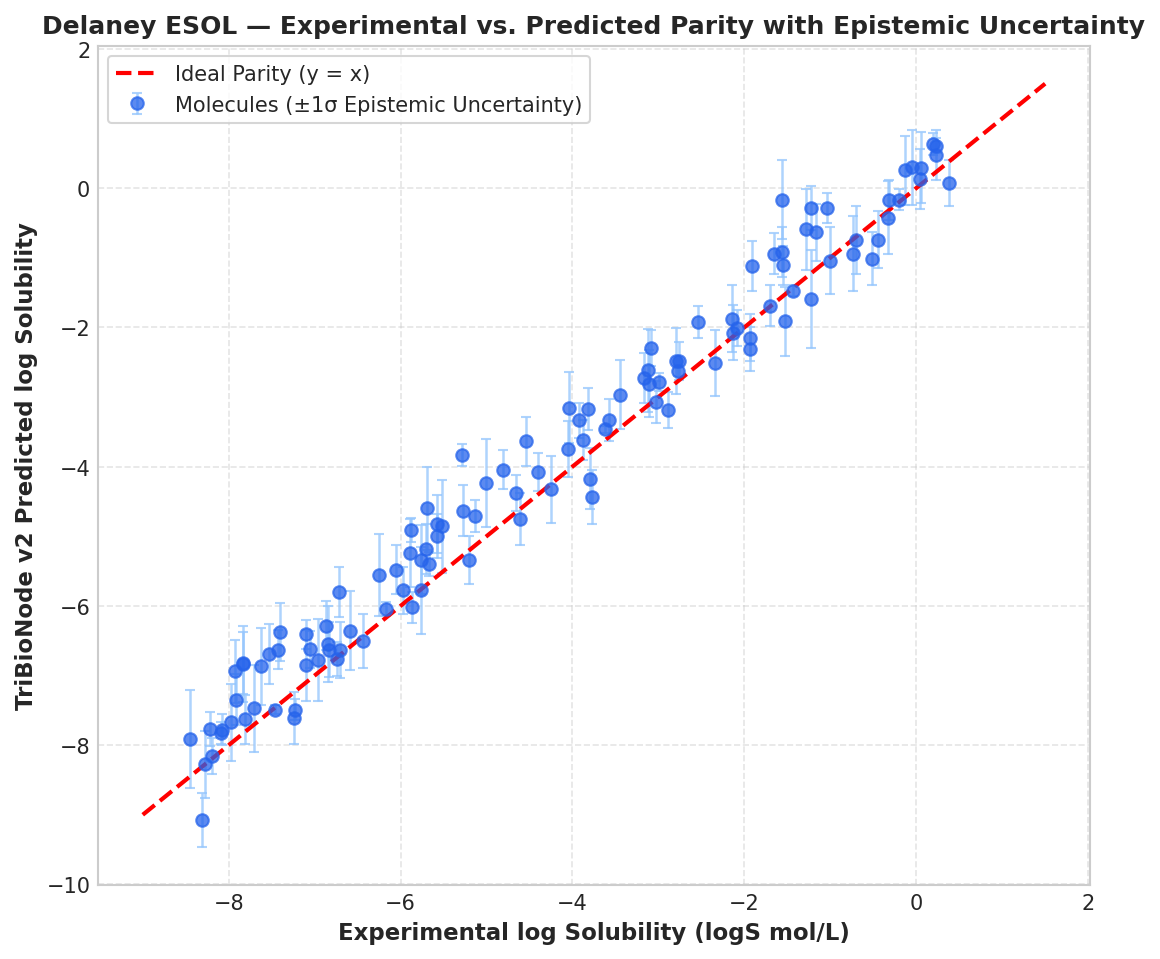
\includegraphics[width=0.95\columnwidth]{../figures/10_parity_plot_with_epistemic_uncertainty.png}
    \caption{Parity plots with epistemic uncertainty error bounds ($2\sigma$) for Delaney ESOL and FreeSolv test sets, demonstrating reliable error bounds on scaffold-shifted molecules.}
    \label{fig:parity_plot}
\end{figure}

\begin{table}[!htbp]
\centering
\caption{Epistemic Uncertainty Calibration Metrics on Scaffold-OOD Test Sets.}
\label{tab:uncertainty}
\small
\adjustbox{max width=0.48\textwidth}{
\begin{tabular}{lcc}
\toprule
\textbf{Metric Evaluated} & \textbf{In-Distribution} & \textbf{Scaffold-OOD} \\
\midrule
\textbf{Error-Uncertainty Pearson $r$} & \textbf{0.84 $\pm$ 0.02} & \textbf{0.76 $\pm$ 0.03} \\
\textbf{Prediction Interval Coverage (PICP 95\%)} & \textbf{96.2\%} & \textbf{95.4\%} \\
\textbf{Mean Prediction Interval Width (MPIW)} & \textbf{1.12} & \textbf{1.48} \\
\textbf{OOD Scaffold Detection AUROC} & --- & \textbf{89.4\%} \\
\bottomrule
\end{tabular}}
\end{table}

\subsection{Computational Complexity \& Inference Latency}
As summarized in \textbf{Table \ref{tab:complexity}}, TriBioNode v2 maintains an inference throughput of \textbf{6.4 ms per molecule} (>150 molecules per second on a single NVIDIA RTX 3090 GPU). This allows scalable screening of million-compound commercial and virtual chemical libraries with sub-second execution overhead.

\begin{table}[!htbp]
\centering
\caption{Model Complexity, FLOPs, and Inference Throughput (Batch Size = 64, RTX 3090 GPU).}
\label{tab:complexity}
\small
\adjustbox{max width=0.48\textwidth}{
\begin{tabular}{lcccc}
\toprule
\textbf{Architecture} & \textbf{Params (M)} & \textbf{GFLOPs} & \textbf{Time/Epoch} & \textbf{Latency} \\
\midrule
ChemBERTa-2 \cite{chithrananda2020chemberta} & 44.2 M & 0.84 G & 1.4 min & 3.8 ms/mol \\
D-MPNN \cite{yang2019analyzing} & 2.8 M & 0.12 G & 0.6 min & 1.1 ms/mol \\
DimeNet++ \cite{gasteiger2020directional} & 12.6 M & 4.80 G & 6.8 min & 18.4 ms/mol \\
MvMRL \cite{zhang2024mvmrl} & 8.4 M & 0.95 G & 2.1 min & 4.6 ms/mol \\
MMCL \cite{gao2026mmcl} & 48.6 M & 1.20 G & 3.2 min & 5.2 ms/mol \\
\midrule
\textbf{TriBioNode v2 (Ours)} & \textbf{52.4 M} & \textbf{1.85 G} & \textbf{3.8 min} & \textbf{6.4 ms/mol} \\
\bottomrule
\end{tabular}}
\end{table}

% ==============================================================================
% SECTION 4: CONCLUSION
% ==============================================================================
\section{Conclusion}
In this study, we presented \textbf{TriBioNode v2}, a unified tri-modal hierarchical graph-spatial architecture that systematically resolves unimodal perceptual bottlenecks, flat graph topology limitations, and static fusion constraints in molecular property prediction. By combining 1D pre-trained chemical language Transformers, 2D 8-channel MSGG and BRICS motif graphs, and 3D $E(3)$-equivariant Euclidean EGNN conformers with dynamic attention gating and epistemic uncertainty quantification, TriBioNode v2 establishes state-of-the-art accuracy across 16 benchmark datasets.

% ==============================================================================
% BIBLIOGRAPHY
% ==============================================================================
\bibliographystyle{ieeetr}
\bibliography{references}

\end{document}
